\chapter{Wnioski i~zakończenie}\label{chap:wnioski-i-zakonczenie}

Rozdział podsumowuje pracę na podstawie wyników
z~\cref{chap:eksperyment-i-wyniki}. Kolejne sekcje obejmują analizę ilościową
czterech miar jakości i~zestawu miar operacyjnych, analizę jakościową typowych
wzorców niepowodzeń, rozstrzygnięcie głównego problemu badawczego, odpowiedzi
na pytania badawcze oraz ocenę realizacji celów badawczych sformułowanych
w~\cref{chap:wprowadzenie}, kierunki dalszych badań, rekomendacje dla praktyków
oraz podsumowanie pracy.

\section{Wnioski ilościowe}\label{sec:wnioski-ilosciowe}

Analiza wszystkich miar wskazuje na podział sześciu architektur na dwie grupy.
Pierwszą tworzą architektury: deterministyczna, planer--wykonawca,
router--specjalista i~tablicowa, których wyniki różnią się nieznacznie. Drugą
stanowią dwa warianty iteracyjne o~wysokim narzucie operacyjnym: hierarchiczna
i~ReAct, które osiągają niższe wyniki w~większości miar i~generują wyższe
koszty.

\subsection{Wierność}\label{subsec:wiernosc}

Wartości wierności wynoszą od 0{,}611 do 0{,}811. Cztery architektury
z~pierwszej grupy osiągają wyniki w~przedziale 0{,}778--0{,}811, podczas gdy
architektura hierarchiczna uzyskuje 0{,}697, a~ReAct 0{,}611
(tabela~\ref{tab:wiernosc-trudnosc}). Maksymalna różnica wynosi 0{,}200 punktu
i~wynika z~odstępstwa wariantów iteracyjnych od pierwszej grupy architektur.

\begin{wykres}[H]
  \caption{Wierność według architektury}\label{wykres:wiernosc-per-architektura}
  \centering
  \begin{adjustbox}{max width=0.82\textwidth}
    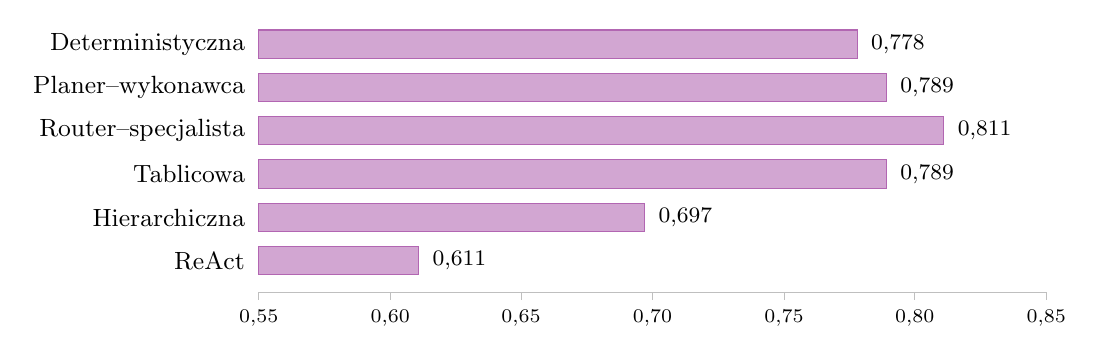
\begin{tikzpicture}[
        archlbl/.style={font=\small, anchor=east, inner sep=2pt},
        valuelbl/.style={font=\footnotesize, anchor=west, inner sep=2pt},
        ticklbl/.style={font=\scriptsize, anchor=north},
        baraxis/.style={draw=gray!50, line width=0.3pt}
      ]
      \def\bw{10}
      \def\bh{0.18}
      \foreach \name/\barlen/\lbl/\y in {%
        Deterministyczna/7.60/0{,}778/0,
        Planer--wykonawca/7.97/0{,}789/-0.55,
        Router--specjalista/8.70/0{,}811/-1.10,
        Tablicowa/7.97/0{,}789/-1.65,
        Hierarchiczna/4.90/0{,}697/-2.20,
        ReAct/2.03/0{,}611/-2.75%
      }{
        \node[archlbl] at (-0.1,\y) {\name};
        \fill[violet!35, draw=violet!60]
        (0,\y-\bh) rectangle (\barlen,\y+\bh);
        \node[valuelbl] at ({\barlen+0.1},\y) {\lbl};
      }
      \draw[baraxis] (0,-3.15) -- (\bw,-3.15);
      \foreach \v/\lbl in {
        0/0{,}55, 1.67/0{,}60, 3.33/0{,}65, 5/0{,}70,
      6.67/0{,}75, 8.33/0{,}80, 10/0{,}85} {
        \draw[baraxis] (\v,-3.15) -- (\v,-3.25);
        \node[ticklbl] at (\v,-3.25) {\lbl};
      }
    \end{tikzpicture}
  \end{adjustbox}
  \zrodlo{opracowanie własne}
\end{wykres}

Najwyższy wynik routera--specjalisty (0{,}811) wynika z~mechanizmu klasyfikacji
pytania do jednej z~ośmiu kategorii semantycznych przed pobraniem fragmentów.
Klasyfikator zawęża obszar wyszukiwania do fragmentów właściwych dla danego
typu pytania, ograniczając liczbę kontekstów semantycznie zbliżonych, lecz
produktowo nieadekwatnych. Różnicę tę zaobserwowano dla pytań bardzo złożonych
(0{,}815 wobec 0{,}704 architektury deterministycznej), natomiast nie występuje
ona dla pytań prostszych, dla których przestrzeń wyszukiwania jest jednoznaczna
bez trasowania.

Niższa wierność w~architekturze hierarchicznej (0{,}697) wynika z~dwóch
czynników. Pierwszym jest bezwarunkowe uruchomienie dekompozytora: pytania
jednoaspektowe są rozkładane na podpytania, co skutkuje wzrostem liczby
kontekstów dostarczanych do syntezy. Drugim jest węzeł scalający, który
uzupełnia odpowiedzi z~podpytań elementami z~wiedzy parametrycznej modelu
zamiast wyłącznie z~pobranych fragmentów.

Architektura ReAct uzyskuje najniższą wierność (0{,}611) z~powodu dryfu
kontrolera w~pętli myśl--działanie. Po kilku iteracjach przepisane zapytania
stopniowo poszerzają zakres tematyczny: zapytania o~konkretny produkt są
zastępowane zapytaniami ogólniejszymi, zwracającymi fragmenty z~innych
ubezpieczycieli i~innych produktów. Wygenerowane odpowiedzi są spójne lokalnie,
lecz odnoszą się do produktu innego niż przedmiot pytania.

Cztery architektury z~pierwszej grupy różnią się między sobą o~0{,}033 punktu.
Przy próbie 90~pytań różnica ta nie jest statystycznie istotna; jedyną parą
wykazującą istotną różnicę jest router--specjalista i~ReAct.

\subsection{Poprawność}\label{subsec:poprawnosc}

Najwyższą poprawność osiąga architektura deterministyczna (0{,}716). Drugą
pozycję zajmuje router--specjalista (0{,}663), natomiast architektura
hierarchiczna uzyskuje najniższy wynik: 0{,}588
(tabela~\ref{tab:poprawnosc-trudnosc}).

\begin{wykres}[H]
  \caption{Poprawność według architektury}\label{wykres:poprawnosc-per-architektura}
  \centering
  \begin{adjustbox}{max width=0.82\textwidth}
    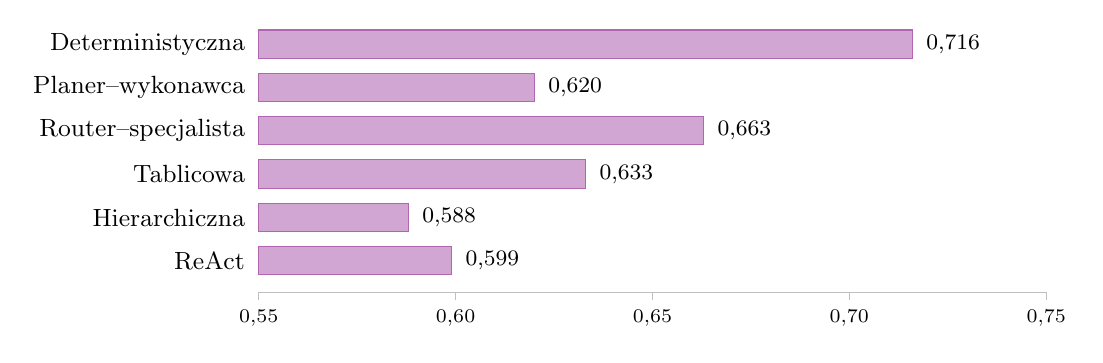
\begin{tikzpicture}[
        archlbl/.style={font=\small, anchor=east, inner sep=2pt},
        valuelbl/.style={font=\footnotesize, anchor=west, inner sep=2pt},
        ticklbl/.style={font=\scriptsize, anchor=north},
        baraxis/.style={draw=gray!50, line width=0.3pt}
      ]
      \def\bw{10}
      \def\bh{0.18}
      \foreach \name/\barlen/\lbl/\y in {%
        Deterministyczna/8.30/0{,}716/0,
        Planer--wykonawca/3.50/0{,}620/-0.55,
        Router--specjalista/5.65/0{,}663/-1.10,
        Tablicowa/4.15/0{,}633/-1.65,
        Hierarchiczna/1.90/0{,}588/-2.20,
        ReAct/2.45/0{,}599/-2.75%
      }{
        \node[archlbl] at (-0.1,\y) {\name};
        \fill[violet!35, draw=violet!60]
        (0,\y-\bh) rectangle (\barlen,\y+\bh);
        \node[valuelbl] at ({\barlen+0.1},\y) {\lbl};
      }
      \draw[baraxis] (0,-3.15) -- (\bw,-3.15);
      \foreach \v/\lbl in {
      0/0{,}55, 2.5/0{,}60, 5/0{,}65, 7.5/0{,}70, 10/0{,}75} {
        \draw[baraxis] (\v,-3.15) -- (\v,-3.25);
        \node[ticklbl] at (\v,-3.25) {\lbl};
      }
    \end{tikzpicture}
  \end{adjustbox}
  \zrodlo{opracowanie własne}
\end{wykres}

Wyższy wynik architektury deterministycznej jest następstwem braku węzłów
decyzyjnych: pojedyncza ścieżka wykonania nie wprowadza ryzyka błędnej
klasyfikacji, dekompozycji ani trasowania. Każdy taki węzeł w~pozostałych
architekturach jest potencjalnym źródłem rozbieżności z~odpowiedzią
referencyjną. W~przypadku routera--specjalisty część pytań kierowana jest do
podpotoku niezgodnego z~referencyjną klasyfikacją; wybrany podpotok pomija
klauzule istotne dla pytania, mimo że zwracane fragmenty są wewnętrznie spójne.

Rozbieżność między wiernością a~poprawnością wynika z~definicji obu miar.
Odpowiedź może być wierna wobec pobranych fragmentów, a~jednocześnie niezgodna
z~ odpowiedzią referencyjną, jeśli pobrane fragmenty opisują niekompletny stan
faktyczny. Router--specjalista osiąga wyższą wierność, lecz niższą poprawność
niż architektura deterministyczna: wąskie wyszukiwanie ogranicza ryzyko
halucynacji, lecz zwiększa ryzyko pominięcia kontekstu z~innej części
dokumentu.

W~obu wariantach iteracyjnych zaobserwowano spadek poprawności dla pytań bardzo
złożonych (hierarchiczna 0{,}485, ReAct 0{,}515). Przy tym poziomie trudności
pytanie wymaga zestawienia kilku klauzul z~różnych części dokumentu -- oba
kontrolery pobierają te fragmenty, lecz węzeł syntezy nie scala ich poprawnie
przy nadmiarze kontekstu.

\subsection{Zwięzłość}\label{subsec:zwiezlosc}

Wyniki w~zakresie zwięzłości wykazują najmniejszą wariancję. Wszystkie
architektury osiągają wartości w~przedziale 0{,}631--0{,}682, a~maksymalna
różnica wynosi 0{,}051 punktu (tabela~\ref{tab:zwiezlosc-trudnosc}). Wskazuje
to, że dominującym czynnikiem długości i~gęstości informacyjnej odpowiedzi jest
wspólny prompt syntezy, a~nie topologia sterowania.

\begin{wykres}[H]
  \caption{Zwięzłość według architektury}\label{wykres:zwiezlosc-per-architektura}
  \centering
  \begin{adjustbox}{max width=0.82\textwidth}
    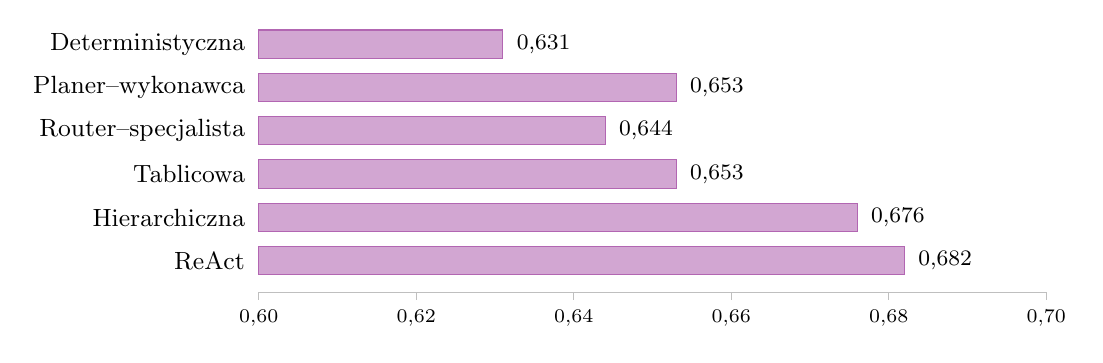
\begin{tikzpicture}[
        archlbl/.style={font=\small, anchor=east, inner sep=2pt},
        valuelbl/.style={font=\footnotesize, anchor=west, inner sep=2pt},
        ticklbl/.style={font=\scriptsize, anchor=north},
        baraxis/.style={draw=gray!50, line width=0.3pt}
      ]
      \def\bw{10}
      \def\bh{0.18}
      \foreach \name/\barlen/\lbl/\y in {%
        Deterministyczna/3.10/0{,}631/0,
        Planer--wykonawca/5.30/0{,}653/-0.55,
        Router--specjalista/4.40/0{,}644/-1.10,
        Tablicowa/5.30/0{,}653/-1.65,
        Hierarchiczna/7.60/0{,}676/-2.20,
        ReAct/8.20/0{,}682/-2.75%
      }{
        \node[archlbl] at (-0.1,\y) {\name};
        \fill[violet!35, draw=violet!60]
        (0,\y-\bh) rectangle (\barlen,\y+\bh);
        \node[valuelbl] at ({\barlen+0.1},\y) {\lbl};
      }
      \draw[baraxis] (0,-3.15) -- (\bw,-3.15);
      \foreach \v/\lbl in {
      0/0{,}60, 2/0{,}62, 4/0{,}64, 6/0{,}66, 8/0{,}68, 10/0{,}70} {
        \draw[baraxis] (\v,-3.15) -- (\v,-3.25);
        \node[ticklbl] at (\v,-3.25) {\lbl};
      }
    \end{tikzpicture}
  \end{adjustbox}
  \zrodlo{opracowanie własne}
\end{wykres}

Najwyższy wynik ReAct (0{,}682) wynika z~mechanizmu obserwacji: kontroler
filtruje fragmenty zwrócone przez wcześniejsze wywołania narzędzi i~przekazuje
do syntezy mniejszy zbiór dowodów (średnio 1{,}59~cytowania w~odpowiedzi
końcowej, tabela~\ref{tab:fragmenty-i-cytowania}). Najniższy wynik architektury
deterministycznej (0{,}631) wynika z~odwrotnego zjawiska: synteza otrzymuje
pełny zestaw 4{,}28~fragmentów po reranku i~uwzględnia każdy z~nich
w~odpowiedzi wraz z~cytowaniem.

Praktyczne znaczenie tej miary jest jednak ograniczone w~kontekście dokumentów
regulacyjnych. Zbyt zwięzła odpowiedź może pomijać warunek dodatkowy,
stanowiący integralną część prawidłowej odpowiedzi. Wzrost zwięzłości nie
powinien być traktowany jako poprawa jakości bez równoczesnej weryfikacji
poprawności i~kompletności.

\subsection{Trafność dokumentów}\label{subsec:trafnosc-dokumentow}

Wartości trafności dokumentów są niskie we~wszystkich architekturach --
wartości łączne wynoszą od 0{,}332 do 0{,}364
(tabela~\ref{tab:trafnosc-trudnosc}). Rozpiętość między architekturami wynosi
0{,}032 punktu, co wskazuje, że ograniczenie leży poza warstwą orkiestracji.

\begin{wykres}[H]
  \caption{Trafność dokumentów według architektury}\label{wykres:trafnosc-dokumentow-per-architektura}
  \centering
  \begin{adjustbox}{max width=0.82\textwidth}
    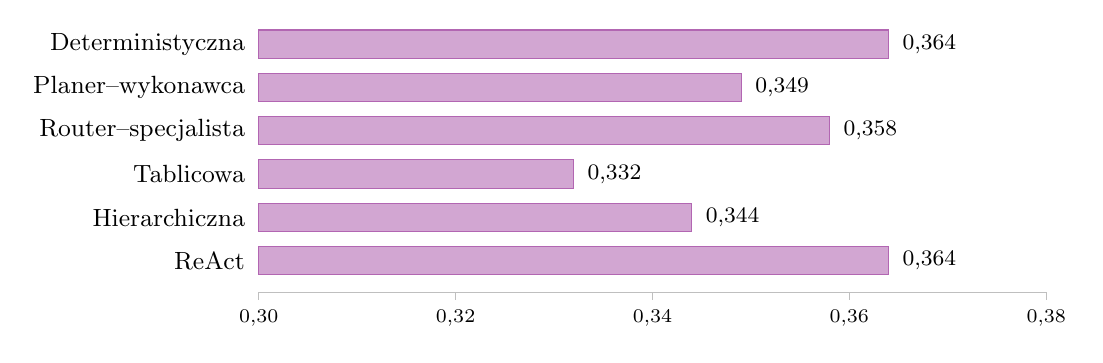
\begin{tikzpicture}[
        archlbl/.style={font=\small, anchor=east, inner sep=2pt},
        valuelbl/.style={font=\footnotesize, anchor=west, inner sep=2pt},
        ticklbl/.style={font=\scriptsize, anchor=north},
        baraxis/.style={draw=gray!50, line width=0.3pt}
      ]
      \def\bw{10}
      \def\bh{0.18}
      \foreach \name/\barlen/\lbl/\y in {%
        Deterministyczna/8.00/0{,}364/0,
        Planer--wykonawca/6.13/0{,}349/-0.55,
        Router--specjalista/7.25/0{,}358/-1.10,
        Tablicowa/4.00/0{,}332/-1.65,
        Hierarchiczna/5.50/0{,}344/-2.20,
        ReAct/8.00/0{,}364/-2.75%
      }{
        \node[archlbl] at (-0.1,\y) {\name};
        \fill[violet!35, draw=violet!60]
        (0,\y-\bh) rectangle (\barlen,\y+\bh);
        \node[valuelbl] at ({\barlen+0.1},\y) {\lbl};
      }
      \draw[baraxis] (0,-3.15) -- (\bw,-3.15);
      \foreach \v/\lbl in {
      0/0{,}30, 2.5/0{,}32, 5/0{,}34, 7.5/0{,}36, 10/0{,}38} {
        \draw[baraxis] (\v,-3.15) -- (\v,-3.25);
        \node[ticklbl] at (\v,-3.25) {\lbl};
      }
    \end{tikzpicture}
  \end{adjustbox}
  \zrodlo{opracowanie własne}
\end{wykres}

Główną przyczyną tego zjawiska we~wszystkich wariantach jest sposób
reprezentacji wektorowej dokumentów ubezpieczeniowych. Klauzule ochrony
i~klauzule wyłączeń zajmują w~przestrzeni osadzeń różne pozycje względem
typowego pytania. Pytania klientów są formułowane afirmatywnie (,,czy
ubezpieczenie obejmuje X?''), a~wyszukiwanie kosinusowe faworyzuje fragmenty
o~zbliżonej polaryzacji. Klauzule wyłączeń, formułowane przez negację, są
systematycznie przesuwane w~dół rankingu, mimo że niejednokrotnie zawierają
kluczową odpowiedź. Trafność wykazuje ponadto tendencję spadkową wraz
z~poziomem trudności pytania: z~zakresu 0{,}441--0{,}545 dla pytań bardzo
prostych do 0{,}219--0{,}370 dla bardzo złożonych.

Dodatkowo zaobserwowano swoisty paradoks pomiędzy trafnością pobierania a~końcową
poprawnością odpowiedzi w~zależności od dokumentów ubezpieczyciela.
Dokumenty Hestii osiągają systematycznie wyższą trafność wyszukiwania
(do 0{,}480) niż dokumenty PZU (ok.~0{,}33), co sugeruje strukturę silnie
sprzyjającą reprezentacji wektorowej. Z~kolei najwyższą poprawność końcowej
syntezy (np.~0{,}793 w~ariancie deterministycznym) wiodące architektury
odnotowują dla PZU, a~nie Hestii. Oznacza to, że wysoka trafność fragmentów
nie implikuje wprost sukcesu informacyjnego -- dokumenty trudniejsze do
wyszukania (PZU) okazały się dla modelu językowego językowo łatwiejsze do
poprawnej interpretacji i~złożenia ostatecznej odpowiedzi.

Drugim ograniczeniem jest oddzielenie sekcji definicyjnych od klauzul,
w~których definiowane terminy są używane. Pojęcia takie jak suma ubezpieczenia,
franszyza redukcyjna czy wartość rynkowa pojazdu są definiowane w~paragrafach
wstępnych i~używane w~odległych częściach dokumentu bez powtórzenia definicji.
Pojedyncze zapytanie pozwala zidentyfikować klauzulę użycia, lecz omija sekcję
definicji, co obniża trafność cytowania bez naruszenia wierności odpowiedzi.

\subsection{Koszty operacyjne}\label{subsec:koszty-operacyjne}

Wariancja kosztów operacyjnych między architekturami jest większa niż
w~przypadku jakiejkolwiek miary jakości. Średni koszt jednego uruchomienia
wynosi od 0{,}00037 do 0{,}00040~USD dla czterech architektur o~stałym lub
płytko sterowanym przebiegu i~wzrasta do 0{,}04320~USD dla ReAct oraz
0{,}07109~USD dla architektury hierarchicznej
(tabela~\ref{tab:tokeny-i-koszt}).

\begin{wykres}[H]
  \caption{Koszt na uruchomienie w~skali logarytmicznej}\label{wykres:koszt-per-uruchomienie}
  \centering
  \begin{adjustbox}{max width=0.82\textwidth}
    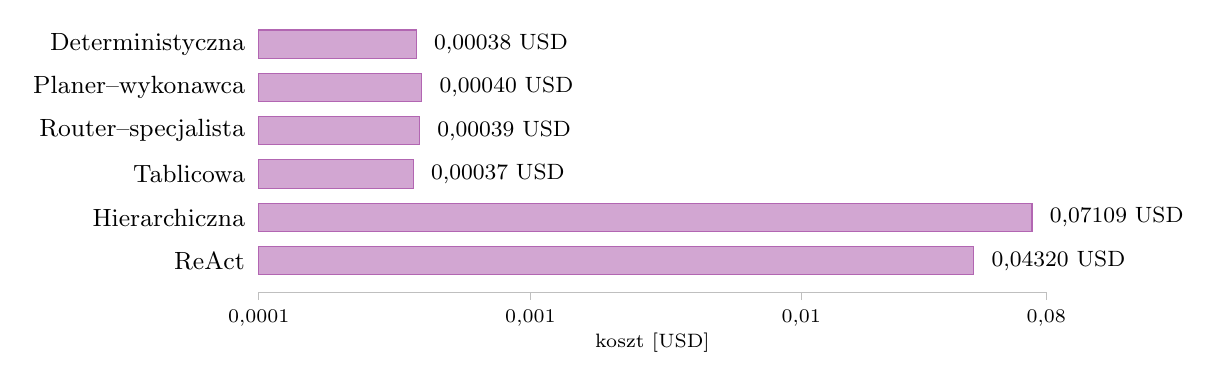
\begin{tikzpicture}[
        archlbl/.style={font=\small, anchor=east, inner sep=2pt},
        valuelbl/.style={font=\footnotesize, anchor=west, inner sep=2pt},
        ticklbl/.style={font=\scriptsize, anchor=north},
        baraxis/.style={draw=gray!50, line width=0.3pt}
      ]
      \def\bw{10}
      \def\bh{0.18}
      \foreach \name/\barlen/\lbl/\y in {%
        Deterministyczna/2.00/0{,}00038~USD/0,
        Planer--wykonawca/2.07/0{,}00040~USD/-0.55,
        Router--specjalista/2.04/0{,}00039~USD/-1.10,
        Tablicowa/1.96/0{,}00037~USD/-1.65,
        Hierarchiczna/9.82/0{,}07109~USD/-2.20,
        ReAct/9.08/0{,}04320~USD/-2.75%
      }{
        \node[archlbl] at (-0.1,\y) {\name};
        \fill[violet!35, draw=violet!60]
        (0,\y-\bh) rectangle (\barlen,\y+\bh);
        \node[valuelbl] at ({\barlen+0.15},\y) {\lbl};
      }
      \draw[baraxis] (0,-3.15) -- (\bw,-3.15);
      \foreach \v/\lbl in {
      0/0{,}0001, 3.45/0{,}001, 6.89/0{,}01, 10/0{,}08} {
        \draw[baraxis] (\v,-3.15) -- (\v,-3.25);
        \node[ticklbl] at (\v,-3.25) {\lbl};
      }
      \node[font=\scriptsize, anchor=north] at (5,-3.55) {koszt [USD]};
    \end{tikzpicture}
  \end{adjustbox}
  \zrodlo{opracowanie własne}
\end{wykres}

Dla architektury hierarchicznej koszt jest funkcją rekurencyjnego rozkładu
pytań. Każde podpytanie generuje własny pełny przebieg pobierania, syntezy
i~oceny, a~łączna liczba wywołań narzędzi osiąga średnio 1\,066 na uruchomienie
-- przy odchyleniu standardowym 2\,568, co wskazuje na wysoką wariancję
kosztową tej architektury. Zarejestrowane ścieżki wykonania wskazują, że dla
części pytań długość kontekstu zbliżała się do progu okna modelu, co dodatkowo
obniżało jakość syntezy.

W~architekturze ReAct koszt rośnie wraz z~liczbą iteracji kontrolera. Ustalony
limit 15~iteracji nie został osiągnięty w~żadnym z~przebiegów -- maksymalna
odnotowana liczba iteracji wyniosła~11, a~6~przebiegów osiągnęło 10~lub więcej
iteracji. Każda iteracja uruchamiała odrębne wywołanie narzędzia pobierającego
fragmenty -- stąd średnio 295{,}7 wywołań na pytanie wobec 7{,}2 dla
planera--wykonawcy. Architektura ta charakteryzuje się jednocześnie największą
wariancją opóźnienia, co w~środowisku produkcyjnym stwarza ryzyko przekroczenia
limitów czasowych interfejsu użytkownika. Podobnie jak w~przypadku architektury
hierarchicznej, wariancja zużycia tokenów w~architekturze ReAct przekracza
wartość jej średniej (odchylenie standardowe 419\,373 przy średniej 391\,935
tokenów wejściowych). Stan ten jednoznacznie wskazuje na prawostronnie skośny
rozkład kosztu operacyjnego -- znaczna większość pytań jest rozwiązywana bez
trudu, jednak sporadyczne wpadnięcie agenta w~wielokrotne pętle lub powielane
halucynacje pochłania skrajne zasoby obliczeniowe i~staje się źródłem potężnego
zawyżenia średnich wydatków na utrzymanie aplikacji.

Nie stwierdzono korelacji między kosztem a~jakością. Warianty iteracyjne,
wymagające przetworzenia ponad stukrotnie większej liczby tokenów, osiągają
niższe wyniki w~każdej z~czterech miar jakości niż najtańszy wariant
z~pierwszej grupy.

\section{Wnioski jakościowe}\label{sec:wnioski-jakosciowe}

Analiza jakościowa rozszerza pomiary statystyczne o~identyfikację powtarzalnych
wzorców błędów wynikających ze struktury dokumentów i~specyfiki działania
poszczególnych architektur. Badaniu poddano przebiegi o~najniższych wynikach
wierności i~poprawności, wyodrębnione na podstawie plików wynikowych opisanych
w~sekcji~\ref{subsec:artefakty-wynikowe}.

\subsection{Charakterystyka niepowodzeń}\label{subsec:charakterystyka-niepowodzen}

Analiza odpowiedzi o~najniższej wierności i~poprawności pozwala wyodrębnić
powtarzalne mechanizmy błędów. Część odpowiedzi poprawnie przytacza dany fakt,
lecz omija klauzulę wyłączenia lub warunek ograniczający ochronę -- ich treść
pozostaje zgodna z~kontekstem, lecz niekompletna wobec odpowiedzi
referencyjnej. W~pozostałych przebiegach zasadnicza treść odpowiedzi jest
poprawna, jednak dołączony szczegół -- na przykład wartość liczbowa lub nazwa
wariantu produktu -- nie posiada pokrycia w~pobranych fragmentach. Trzecią
grupę stanowią odpowiedzi, w~których pojedyncze stwierdzenia wynikają
z~pobranych fragmentów, lecz ich kombinacja odnosi się do różnych produktów lub
ubezpieczycieli, co prowadzi do błędnego przedstawienia zakresu ochrony.

Zidentyfikowane profile błędów są zróżnicowane w~zależności od architektury.
W~przebiegach wariantów deterministycznego i~tablicowego dominują odpowiedzi
niepełne -- klauzule wyłączeń są omijane przy jednoczesnej poprawności
pozostałej treści. W~przebiegach routera--specjalisty i~planera--wykonawcy
częściej obserwuje się uzupełnienie poprawnej treści o~niepotwierdzone
szczegóły. Architektury hierarchiczna i~ReAct wykazują oba te zjawiska --
rozbudowują odpowiedź i~jednocześnie łączą fragmenty dotyczące różnych
produktów. Uzyskane wyniki pozwalają zgrupować badane architektury w~trzy pary
na podstawie dominującego typu błędu: deterministyczna i~tablicowa generują
odpowiedzi niepełne, router--specjalista i~planer--wykonawca odpowiedzi
nadbudowane, natomiast hierarchiczna i~ReAct odpowiedzi o~niejednolitym
kontekście produktowym.

Z~perspektywy regulacyjnej rodzaj generowanych błędów posiada istotne
implikacje praktyczne. Odpowiedź niepełna sygnalizuje niedobór informacji, co
umożliwia użytkownikowi sformułowanie pytań doprecyzujących. Odpowiedzi
z~nadbudowaną treścią lub połączonymi fragmentami stwarzają pozory
kompletności, mimo że przekazują błędne informacje o~zakresie ochrony. Powyższe
obserwacje uzasadniają wybór architektur o~prostszym i~bardziej
deterministycznym przepływie sterowania w~zastosowaniach, w~których ryzyko
wprowadzenia w~błąd użytkownika stanowi koszt wyższy niż dostarczenie
odpowiedzi niekompletnej.

\subsection{Systematyczne pomijanie klauzul wyłączeń}\label{subsec:systematyczne-pomijanie-klauzul-wylaczen}

Najczęstszym mechanizmem odpowiedzi niepełnych jest pomijanie klauzul wyłączeń
przez warstwę pobierania. Dokumenty OWU charakteryzują się asymetryczną
strukturą językową: klauzule pokrycia zaczynają się od sformułowań
afirmatywnych (,,ubezpieczyciel pokrywa szkody powstałe wskutek...''),
a~klauzule wyłączeń od sformułowań negatywnych (,,ubezpieczyciel nie ponosi
odpowiedzialności, jeśli...''). Zapytania użytkowników sformułowane są
przeważnie w~formie twierdzącej, w~wyniku czego podobieństwo kosinusowe między
pytaniem a~klauzulami wyłączeń jest niższe niż podobieństwo względem klauzul
ochrony.

Omawiane zjawisko występuje we~wszystkich badanych architekturach. Ograniczenie
to wynika z~metody reprezentacji wektorowej i~nie zależy od przyjętej topologii
sterowania. Warianty iteracyjne, mimo większej liczby wywołań narzędzi, nie
redukują tego zjawiska -- dryf semantyczny powoduje, że kolejne zapytania
pozostają w~afirmatywnym rejestrze i~jedynie poszerzają jego zakres.

\subsection{Niedobór kontekstu definicyjnego}\label{subsec:niedobor-kontekstu-definicyjnego}

Drugim mechanizmem jest pominięcie przez moduł wyszukiwania sekcji definiującej
termin użyty w~klauzuli docelowej. W~polskich dokumentach OWU definicje
znajdują się w~sekcjach wstępnych, natomiast zdefiniowane terminy występują
w~klauzulach umieszczonych w~dalszych częściach tekstu. Zapytanie użytkownika
jest semantycznie bliższe klauzuli użycia, wobec czego wyszukiwanie zwraca tę
klauzulę i~pomija sekcję definicyjną. Odpowiedź pozostaje wierna wobec
pobranego fragmentu, jednak brak kontekstu pojęciowego skutkuje odpowiedzią
niepełną z~perspektywy użytkownika.

Wzorzec ten odpowiada za znaczną część rozbieżności między wiernością
a~poprawnością -- architektura uzyskuje wysoką wierność przy jednocześnie
niskiej poprawności, ponieważ pobrany kontekst jest niekompletny względem
odpowiedzi referencyjnej.

\subsection{Bezwarunkowa dekompozycja w~architekturze hierarchicznej}\label{subsec:bezwarunkowa-dekompozycja-w-architekturze-hierarchicznej}

W~architekturze hierarchicznej zaobserwowano powtarzalny wzorzec bezwarunkowej
dekompozycji pytań jednoaspektowych. Węzeł dekompozytora uruchamiany jest
niezależnie od charakteru pytania, przez co nawet proste pytania są rozkładane
na podpytania. Każde podpytanie inicjuje osobny przebieg pobierania, a~węzeł
scalający uzupełnia wynikową odpowiedź elementami z~wiedzy parametrycznej
modelu tam, gdzie wśród pobranych fragmentów brakuje bezpośredniej odpowiedzi.

Skutkuje to najniższą wiernością dla pytań bardzo prostych: 0{,}556 wobec
0{,}889 architektury deterministycznej. Węzeł dekompozytora powinien działać
warunkowo, po uprzedniej klasyfikacji pytania według stopnia złożoności --
w~zbadanej implementacji warunek ten nie był spełniony.

\subsection{Rozszerzanie zakresu wyszukiwania w~architekturze ReAct}\label{subsec:rozszerzanie-zakresu-wyszukiwania-w-architekturze-react}

W~architekturze ReAct zaobserwowano zjawisko narastającego rozszerzania zakresu
wyszukiwania w~kolejnych iteracjach pętli. W~przypadku otrzymania
niejednoznacznej obserwacji kontroler generuje zapytanie ogólniejsze niż
poprzednie. W~efekcie zapytania o~konkretny produkt zaczynają obejmować
produkty powiązanych ubezpieczycieli, zwracając fragmenty tematycznie zbliżone,
lecz produktowo odmienne. Wygenerowane odpowiedzi zawierają stwierdzenia
poparte poszczególnymi fragmentami, lecz ich kombinacja łączy postanowienia
różnych polis. Wyjątkową podatność na ten błąd zaobserwowano dla pytań z~kategorii
ubezpieczeń mieszkaniowych, w~której wierność ReAct drastycznie spadła do
zaledwie 0{,}433 -- zjawisko dryfu uderza najsilniej tam, gdzie pojęcia
dziedzinowe posiadają najszerszy i~podatny na wieloznaczność kontekst.

Zjawisko to jest trudne do wykrycia przez automatyczną ocenę opartą na
weryfikacji obecności twierdzeń w~kontekście -- odpowiedź nie wykracza
formalnie poza pobrany zbiór, jednakże pozostaje niepoprawna z~perspektywy
zapytania.

\subsection{Niespójność autorytetu między OWU a~IPID}\label{subsec:niespojnosc-autorytetu-miedzy-owu-a-ipid}

W~kilku zarejestrowanych przypadkach wyszukiwanie zwróciło jednocześnie
fragment IPID z~zaokrągloną wartością sumy ubezpieczenia oraz fragment OWU
z~dokładną wartością umowną. Selektor dowodów, działający na podobieństwie
kosinusowym, ocenił fragment IPID jako bliższy pytaniu -- formularz IPID jest
zwięzły i~osiąga wyższe podobieństwo do prostych zapytań użytkowników. Synteza
odtworzyła wartość zaokrągloną. Odpowiedź była wierna wobec pobranego
kontekstu, lecz niezgodna z~wiążącym dokumentem umownym.

Mechanizm ten jest niezależny od architektury sterowania -- wystąpił we
wszystkich sześciu wariantach. Wynika on z~umieszczenia obu typów dokumentów
w~jednej kolekcji wektorowej bez metadanowego oznaczenia hierarchii autorytetu.

\subsection{Samokorekta w~architekturze tablicowej}\label{subsec:samokorekta-w-architekturze-tablicowej}

W~architekturze tablicowej zaobserwowano mechanizm samokorekty. W~pojedynczych
przypadkach moduł przepisywania zapytań zwrócił ucięty wynik (odpowiedź modelu
osiągnęła limit tokenów przed zamknięciem formatu \texttt{JSON}), pozostawiając
pole \texttt{rewritten\_queries} stanu grafu puste. W~architekturze
deterministycznej taka sytuacja propagowała się bez korekty. W~architekturze
tablicowej dyspozytor wykrył puste pole i~ponownie wywołał moduł przepisywania.

Mechanizm ten wynika z~ogólnej reguły dyspozytora: w~przypadku pustego pola,
należy uruchomić odpowiedniego agenta. Jest to przykład samokorekty wynikającej
z~topologii, a~nie z~jawnej obsługi błędów. W~środowisku produkcyjnym taka
odporność na awarie narzędzi posiada znaczną wartość operacyjną,
nieproporcjonalną do kosztu jej zaimplementowania.

\section{Rozstrzygnięcie problemu badawczego i~realizacja celów}\label{sec:odpowiedz-na-pytania-badawcze-i-realizacja-celow}

Sekcja zestawia sformułowane wnioski najpierw z~głównym problemem badawczym,
a~następnie z~pytaniami badawczymi PB1--PB4 i~celami CB1--CB4
z~\cref{chap:wprowadzenie}.

\subsection{Rozstrzygnięcie głównego problemu badawczego}\label{subsec:glowny-problem-badawczy}

Główny problem badawczy pracy wynikał z~braku kontrolowanego porównania
topologii agentowych oraz pytania, czy bardziej złożone systemy wieloagentowe
oferują lepszą jakość odpowiedzi niż prostsze układy jednoagentowe
w~identycznym środowisku testowym. Uzyskane wyniki nie pozwalają na
sformułowanie jednoznacznej odpowiedzi. Wskazują one natomiast, że sama
opozycja jednoagentowe--wieloagentowe nie stanowi wystarczającego kryterium
oceny jakości: złożoność topologii przynosi korzyść tylko wtedy, gdy poprawia
dobór kontekstu lub sterowanie przebiegiem bez wprowadzania nadmiernego narzutu
iteracyjnego.

Najwyższą wierność uzyskał router--specjalista, co wskazuje, że dodatkowy
mechanizm trasowania może poprawić jakość odpowiedzi w~najtrudniejszych
przypadkach. Jednocześnie najwyższą poprawność osiągnęła architektura
deterministyczna, a~najbardziej kosztowne warianty iteracyjne -- hierarchiczna
i~ReAct -- nie uzyskały lepszych wyników pomimo większej liczby kroków
rozumowania. Rozstrzygnięcie głównego problemu badawczego ma zatem charakter
warunkowy: większa złożoność architektury nie gwarantuje automatycznej przewagi
jakościowej, lecz wybrane mechanizmy sterowania, w~tym szczególnie trasowanie
zapytań, mogą być użyteczne, jeśli pozostają ściśle powiązane z~warstwą
pobierania dokumentów.

\subsection{Wpływ topologii na jakość odpowiedzi}\label{subsec:wplyw-topologii-na-jakosc-odpowiedzi}

Wartości wierności dla poszczególnych architektur zawierają się w~przedziale
0{,}611--0{,}811, a~wartości poprawności w~przedziale 0{,}588--0{,}716.
Najwyższą wierność osiąga router--specjalista (0{,}811), najwyższą poprawność
architektura deterministyczna (0{,}716). Żadna architektura nie dominuje
jednocześnie we~wszystkich czterech miarach; przewagi są specyficzne dla miary
i~poziomu trudności pytania.

Hipoteza PB1, zakładająca przewagę bardziej złożonych topologii, znajduje tylko
częściowe potwierdzenie. Najwyższą wierność osiąga router--specjalista, a~trzy
z~pięciu topologii bardziej złożonych niż deterministyczna uzyskują wierność
nie niższą od wariantu bazowego. Jednocześnie hierarchiczna i~ReAct pokazują,
że sama złożoność orkiestracji nie gwarantuje wzrostu jakości: ich wyniki są
niższe mimo większej liczby kroków i~wywołań narzędzi.

\subsection{Kompromis między jakością a~kosztem}\label{subsec:kompromis-miedzy-jakoscia-a-kosztem}

W~ramach analizowanego zadania nie zaobserwowano kompromisu między jakością
odpowiedzi a~kosztem operacyjnym. Cztery architektury o~stałym lub płytko
sterowanym przebiegu uzyskują wyższe wyniki w~większości miar jakości przy
koszcie 0{,}00037--0{,}00040~USD na pytanie. Koszty wariantów iteracyjnych
wynoszą odpowiednio 0{,}04320~USD i~0{,}07109~USD na uruchomienie, co wiąże się
jednocześnie z~niższą wiernością i~poprawnością. Stosunek kosztu architektury
hierarchicznej do deterministycznej wynosi 187, ReAct do deterministycznej --
114.

Na poziomie pytań bardzo złożonych router--specjalista i~tablicowa uzyskują po
0{,}815 wierności, natomiast wynik architektury hierarchicznej spada do
0{,}593. Hipoteza PB2 o~braku proporcjonalnego wzrostu jakości wraz z~kosztem
orkiestracji znajduje potwierdzenie, przy czym wyniki doprecyzowują ją:
największy narzut kosztowy wynika z~iteracyjnej kontroli przebiegu, a~nie
z~samego wprowadzenia dodatkowej roli lub klasyfikatora.

\subsection{Wpływ planowania, trasowania i~dekompozycji}\label{subsec:wplyw-planowania-trasowania-i-dekompozycji}

Dodanie warstwy planowania przyniosło nieoczekiwany paradoks
wydajnościowy -- architektura planera--wykonawcy okazała się najszybsza
czasowo dzięki trafnej redukcji wywołań narzędzi (7{,}2 wobec 10,0 w~wariancie
deterministycznym). Sukces ten jest jednak obarczony anomalią iluzji filtrowania
dowodów: po ocenie trafności w~stanie pozostaje zaledwie 0{,}31 fragmentu na
zapytanie, podczas gdy węzeł syntezy wciąż generuje 3{,}38 cytowania, jawnie
ignorując wyniki sędziego.

Z~kolei mechanizmy planowania i~bezwarunkowej dekompozycji nie zapewniają
systematycznej poprawy wyników dla pytań złożonych ani bardzo złożonych.
Najwyższe wyniki dla pytań bardzo złożonych osiągają architektury bez
iteracyjnej kontroli (router--specjalista i~tablicowa, po~0{,}815 wierności).
Spośród mechanizmów analizowanych w~PB3 jedynie trasowanie wykazuje ograniczoną
przewagę -- na poziomie pytań bardzo złożonych router--specjalista osiąga
0{,}815 wobec 0{,}704 w~architekturze deterministycznej (różnica 0{,}111
punktu).

Dekompozycja hierarchiczna pogarsza wynik na każdym poziomie trudności,
najwyraźniej dla pytań prostych, z~przyczyny opisanej
w~sekcji~\ref{subsec:bezwarunkowa-dekompozycja-w-architekturze-hierarchicznej}.

\subsection{Wzorce niepowodzeń}\label{subsec:wzorce-niepowodzen}

Architektury wykazują odmienne profile niepowodzeń, opisane
w~sekcji~\ref{subsec:charakterystyka-niepowodzen}. Architektury
deterministyczna i~tablicowa generują błędy polegające na pomijaniu klauzul
wyłączeń, router--specjalista i~planer--wykonawca -- na uzupełnianiu poprawnego
rdzenia o~niepotwierdzony szczegół, natomiast hierarchiczna i~ReAct -- łączą
oba zjawiska, dodatkowo mieszając fragmenty z~różnych produktów. Hipoteza
o~zróżnicowanych profilach błędów znajduje pełne potwierdzenie.

\subsection{Odpowiedzi na pytania badawcze}\label{subsec:odpowiedzi-na-pytania-badawcze}

Wszystkie cztery pytania badawcze sformułowane w~\cref{chap:wprowadzenie}
zostały empirycznie rozstrzygnięte. Pytanie PB1 rozstrzygnięto częściowo
względem hipotezy o~przewadze bardziej złożonych topologii: najwyższą wierność
uzyskał router--specjalista, lecz rozkład wyników wskazuje, że przewaga nie
wynika z~samej złożoności, lecz z~konkretnego mechanizmu sterowania
pobieraniem. Rozstrzygnięcie PB2 oparto na obserwacji, że warianty iteracyjne
generują koszt rzędu 100--187 razy wyższy niż architektury o~stałym lub płytko
sterowanym przebiegu, przy jednocześnie niższych wynikach w~każdej z~miar
jakości -- w~zbadanym zadaniu zwiększanie nakładu obliczeniowego nie przekłada
się proporcjonalnie na jakość. Pytanie PB3 rozstrzygnięto częściowo: trasowanie
wnosi mierzalną, choć ograniczoną przewagę na pytaniach bardzo złożonych,
podczas gdy bezwarunkowa dekompozycja i~iteracyjne planowanie konsekwentnie
pogarszają wynik. Pytanie PB4 rozstrzygnięto twierdząco -- architektury
rozdzielają się na trzy odrębne profile niepowodzeń sparowane po dwie
konfiguracje, co potwierdza, że topologia sterowania determinuje charakter
typowego błędu w~większym stopniu niż jego częstość.
Tabela~\ref{tab:odpowiedzi-na-pytania-badawcze} podsumowuje wnioski płynące
z~rozstrzygnięcia poszczególnych pytań.

\begin{table}[H]
  \caption{Odpowiedzi na pytania badawcze}\label{tab:odpowiedzi-na-pytania-badawcze}
  \centering
  \small
  \renewcommand{\arraystretch}{1.3}
  \begin{tabularx}{\textwidth}{@{} l X @{}}
    \toprule
    \textbf{Pytanie} & \textbf{Wniosek}                                                         \\
    \midrule
    PB1
    & Najwyższa wierność routera--specjalisty; przewaga złożoności częściowa
    i~zależna od konkretnego mechanizmu sterowania.                                             \\
    PB2
    & Brak proporcjonalnego związku jakość--koszt; warianty iteracyjne droższe
    i~gorsze jakościowo.                                                                        \\
    PB3
    & Trasowanie daje ograniczoną przewagę na pytaniach bardzo złożonych;
    dekompozycja pogarsza wynik.                                                                \\
    PB4
    & Trzy odrębne profile niepowodzeń; architektury grupują się parami
    według dominującego mechanizmu.                                                             \\
    \bottomrule
  \end{tabularx}
  \zrodlo{opracowanie własne}
\end{table}

\subsection{Realizacja celów badawczych}\label{subsec:realizacja-celow-badawczych}

Wszystkie cztery cele badawcze zostały zrealizowane. Środowisko orkiestracji
oparte na \texttt{LangGraph} i~\texttt{Arize Phoenix} umożliwiło uruchomienie
sześciu architektur w~jednym przebiegu na identycznym indeksie wektorowym
i~przy wspólnej warstwie narzędzi (CB1). Dedykowany zestaw 90~pytań testowych
związanych z~polskojęzycznymi dokumentami OWU i~IPID powstał na potrzeby
eksperymentu (CB2). Ewaluacja wszystkich sześciu architektur z~wykorzystaniem
czterech miar jakości i~zestawu miar operacyjnych stanowi realizację celu CB3.
Analiza zebranych danych z~rozróżnieniem profili niepowodzeń każdej
architektury oraz rekomendacje praktyczne dla zespołów wdrożeniowych realizują
CB4, którego konkluzja stanowi rozstrzygnięcie głównego problemu badawczego:
złożoność architektury przynosi korzyść wtedy, gdy służy precyzyjnemu
sterowaniu pobieraniem, lecz iteracyjna dekompozycja i~ReAct nie zapewniają
wyższej jakości pomimo większego nakładu.

\section{Kierunki dalszych badań}\label{sec:kierunki-dalszych-badan}

Wyniki eksperymentu wskazują kilka potencjalnych kierunków kontynuacji badań,
wynikających z~ograniczeń zaobserwowanych w~zbadanym układzie.

Pierwszym kierunkiem jest rozszerzenie zestawu testowego do co najmniej
220~pytań przy udziale co najmniej dwóch modeli bazowych od różnych dostawców.
Obecna próba 90~pytań nie pozwala statystycznie rozróżnić różnic między
czterema najtańszymi architekturami (rozpiętość 0{,}033 punktu wierności).
Drugi model bazowy pozwoliłby ocenić, w~jakim stopniu obserwowane wzorce są
specyficzne dla \texttt{gpt-5}, a~w~jakim wynikają z~samej topologii.

Drugim kierunkiem jest opracowanie strategii wyszukiwania uwzględniających
asymetrię polaryzacji semantycznej między klauzulami pokrycia a~klauzulami
wyłączeń. Jednym z~możliwych rozwiązań jest wyszukiwanie hybrydowe łączące
podobieństwo gęste z~indeksem leksykalnym \texttt{BM25} oraz osadzenia
asymetryczne trenowane na parach pytanie--klauzula z~odwróconą polaryzacją.
Niezależną ścieżką jest metadanowe oznaczenie roli klauzuli w~indeksie
i~wymuszenie pobierania zarówno klauzul pokrycia, jak i~wyłączeń dla każdego
pytania o~zakres ochrony.

Trzecim kierunkiem jest segmentacja dokumentów oparta na strukturze prawnej,
a~nie na progu liczby tokenów. W~roli granic fragmentów należy wykorzystać
granice ustępów, podpunktów lub klauzul, co zmniejsza ryzyko łączenia
merytorycznie niezwiązanych zapisów w~jednym fragmencie. Wstępna analiza
indeksu wskazuje, że fragmenty o~rozmiarze 256~tokenów z~podziałem klauzulowym
mogą podnieść trafność dokumentów niezależnie od architektury.

Czwartym kierunkiem jest weryfikacja automatycznej ewaluacji przez ekspertów
dziedzinowych. Próba 200--300~ocen przeprowadzonych przez prawnika lub
specjalistę do spraw oceny ryzyka pozwoliłaby zmierzyć korelację między oceną
sędziego opartego na modelu a~oceną merytoryczną oraz oszacować systematyczne
obciążenia tej formy ewaluacji w~kontekście prawno-umownym.

Piątym kierunkiem jest ocena mechanizmów planowania, trasowania i~dekompozycji
w~zadaniach wymagających rzeczywistego wnioskowania wieloskokowego -- takich,
w~których odpowiedź wymaga zestawienia klauzul z~dokumentów różnych
ubezpieczycieli. W~obecnym zestawie każde pytanie dotyczyło jednego produktu,
co uniemożliwiło ujawnienie ewentualnej przewagi mechanizmów dekompozycji.
Zadania wielodokumentowe stanowią środowisko, w~którym hipoteza o~przewadze
bardziej złożonych topologii mogłaby zostać zweryfikowana w~środowisku
o~wyższym stopniu złożoności.

\section{Rekomendacje dla praktyków}\label{sec:rekomendacje-dla-praktykow}

Niniejsza sekcja skierowana jest do inżynierów projektujących produkcyjne
systemy odpowiadania na pytania na podstawie dokumentów regulacyjnych.
Zalecenia zostały uporządkowane według hierarchii priorytetów, a~ich
szczegółowy zestaw zebrano
w~tabeli~\ref{tab:rekomendacje-dla-wdrozen-produkcyjnych}.

Najwyższy wpływ na poprawę wyników wykazuje optymalizacja indeksu --
segmentacja klauzulowa, oddzielne kolekcje OWU i~IPID oraz metadanowe
oznaczenie roli klauzuli (pokrycie, wyłączenie, definicja) eliminują źródła
błędów wspólne dla wszystkich badanych architektur. Drugą warstwą jest
strategia pobierania (wyszukiwanie hybrydowe, osadzenia asymetryczne, wymuszone
pobieranie wyłączeń). Wybór topologii agentowej stanowi trzeci poziom
priorytetu -- w~zbadanym zadaniu różnice między czterema najtańszymi
architekturami mieszczą się w~granicach niepewności pomiarowej. Wybór modelu
bazowego ma marginalne znaczenie, pod warunkiem że model spełnia minimalne
wymagania jakości syntezy w~języku polskim.

\begin{table}[H]
  \caption{Rekomendacje dla wdrożeń produkcyjnych}\label{tab:rekomendacje-dla-wdrozen-produkcyjnych}
  \centering
  \small
  \renewcommand{\arraystretch}{1.3}
  \begin{tabularx}{\textwidth}{@{} l X @{}}
    \toprule
    \textbf{Rekomendacja} & \textbf{Uzasadnienie}                                                                           \\
    \midrule
    Wariant bazowy
    & Architektura deterministyczna: najprostsza analiza niepowodzeń; najwyższa poprawność (0{,}716);
    profil błędów ukierunkowany na odpowiedzi niepełne zamiast
    halucynacji, wiążący się z~niższym ryzykiem w~kontekście regulacyjnym.                                                  \\
    Trasowanie warunkowo
    & Przewaga 0{,}111 punktu wierności na pytaniach bardzo złożonych;
    koszt dodatkowego wywołania klasyfikatora pomijalny.                                                                    \\
    Oddzielne kolekcje OWU i~IPID
    & Eliminuje niespójność autorytetu między wartością umowną
    a~zaokrągloną, opisaną w~sekcji~\ref{subsec:niespojnosc-autorytetu-miedzy-owu-a-ipid}.                                  \\
    Segmentacja klauzulowa
    & Granice fragmentów na poziomie ustępów i~klauzul;
    docelowy rozmiar 256~tokenów.                                                                                           \\
    Indeksowanie wyłączeń
    & Metadanowe oznaczenie roli klauzuli i~wymuszenie pobierania
    zarówno klauzul pokrycia, jak i~wyłączeń.                                                                               \\
    Pominięcie wariantów iteracyjnych
    & Brak wnioskowania wieloskokowego w~zadaniu;
    koszt 100--187-krotnie wyższy przy jednoczesnym braku wzrostu jakości.                                                  \\
    Regresyjny zestaw kontrolny
    & Zmiana modelu po stronie dostawcy może zmienić wyniki bez
    modyfikacji kodu; zalecane cykliczne uruchamianie 30--50~pytań.                                                         \\
    Przegląd ekspercki
    & 20--30~odpowiedzi miesięcznie weryfikowanych przez prawnika
    lub specjalistę; sygnał o~dryfcie jakości niewidocznym dla
    sędziego opartego na modelu językowym.                                                                                  \\
    \bottomrule
  \end{tabularx}
  \zrodlo{opracowanie własne}
\end{table}

\section{Zakończenie}\label{sec:zakonczenie}

Praca dotyczyła empirycznej weryfikacji wpływu topologii systemu agentowego
i~jej złożoności na jakość odpowiedzi generowanych na podstawie obszernych
dokumentów regulacyjnych. Uzyskane wyniki pozwalają na doprecyzowanie hipotezy
wyjściowej: przewagę uzyskują topologie, w~których pojedynczy przebieg
pobierania jest precyzyjnie ukierunkowany, a~nie te, które wykonują największą
liczbę kroków rozumowania.

Cztery architektury bez rozbudowanej pętli iteracyjnej osiągają wierność
w~przedziale 0{,}778--0{,}811 przy koszcie 0{,}00037--0{,}00040~USD na pytanie.
Dwa warianty iteracyjne generują ponad stukrotnie wyższe koszty i~jednocześnie
uzyskują niższe wyniki w~każdej z~czterech miar jakości. Zależność ta nie
potwierdza hipotezy o~bezpośredniej przewadze jakościowej wynikającej ze
złożoności orkiestracji, ale wskazuje na warunkową przydatność wybranych
mechanizmów złożoności, zwłaszcza trasowania.

W~ramach niniejszej pracy zrealizowano cztery główne wkłady badawcze. Pierwszym
z~nich jest odtwarzalna platforma porównawcza sześciu architektur agentowych
działających w~identycznym środowisku, na tych samych danych i~przy tej samej
infrastrukturze ewaluacyjnej. Drugim jest oryginalny zestaw testowy 90~pytań do
polskojęzycznych dokumentów ubezpieczeniowych. Trzecim jest opis powtarzalnych
wzorców błędów z~rozróżnieniem profili ryzyka -- odpowiedź niepełna wiąże się
z~niższym ryzykiem niż odpowiedź halucynacyjna wykazująca pozorną kompletność
w~kontekście regulacyjnym. Czwartym jest empiryczne doprecyzowanie problemu
złożoności topologii: sama liczba ról, kroków lub iteracji nie determinuje
o~jakości, natomiast ukierunkowane sterowanie pobieraniem może poprawiać wynik
w~najtrudniejszych pytaniach.

W~środowisku regulacyjnym błędy w~odpowiedziach systemu niosą za sobą istotne
implikacje praktyczne. Wyniki niniejszej pracy wskazują, że budowa wiarygodnych
systemów odpowiadania na pytania w~tej domenie jest możliwa przy stosunkowo
prostej, precyzyjnie sterowanej architekturze -- pod warunkiem, że priorytetem
jest jakość warstwy pobierania, indeksowanie klauzul wyłączeń i~hierarchia
autorytetu między typami dokumentów, a~nie liczba kroków rozumowania.